\section{Esercizio 2.1.1}

\subsection{Problem Statement}
\begin{enumerate}
    \item \textbf{Scrivere una funzione} che accetti una matrice triangolare superiore e implementi la backward substitution. Testarla sul sistema lineare $U\mathbf{x} = \mathbf{b}$ con
    \[
        U = \begin{pmatrix} 2 & 1 & 1 \\ 0 & 1 & -2 \\ 0 & 0 & 1 \end{pmatrix}, \quad \mathbf{b} = \begin{pmatrix} 1 \\ -1 \\ 4 \end{pmatrix}
    \]
    e verificare che la soluzione sia corretta.

    \item \textbf{Scrivere una funzione separata} che esegua la Gauss elimination e combinarla con la Backward substitution per risolvere il sistema
    \[
        \begin{pmatrix} 2 & 1 & 1 \\ 1 & 1 & -2 \\ 1 & 2 & 1 \end{pmatrix} \begin{pmatrix} x_0 \\ x_1 \\ x_2 \end{pmatrix} = \begin{pmatrix} 8 \\ -2 \\ 2 \end{pmatrix}
    \]
    Verificare la soluzione. 

    \item \textbf{Utilizzando i programmi precedenti}, aggiungere una funzione che stampi anche l'inversa esplicita di una matrice. Testarla sulla matrice sopra indicata e verificare il risultato.

    \item \textbf{Adattare i programmi precedenti} per includere il partial pivoting e risolvere i seguenti sistemi. Verificare che senza partial pivoting il programma fallisca, poiché in qualche passaggio intermedio appare $A_{jj} = 0$ per la matrice
    \[
        \begin{pmatrix} 2 & 1 & 1 \\ 2 & 1 & -4 \\ 1 & 2 & 1 \end{pmatrix} \begin{pmatrix} x_0 \\ x_1 \\ x_2 \end{pmatrix} = \begin{pmatrix} 8 \\ -2 \\ 2 \end{pmatrix}
    \]

    \item \textbf{Studiare la soluzione} del problema
    \[
        \begin{pmatrix} 10^{-20} & -1 \\ 1 & 1 \end{pmatrix} \begin{pmatrix} x_0 \\ x_1 \end{pmatrix} = \begin{pmatrix} 1 \\ 2 \end{pmatrix}
    \]
    con e senza pivoting. In questo caso il sistema non è mal condizionato (ovvero non genera infiniti), ma produce un risultato errato. Spiegare l'origine dell'errore e perché il pivoting lo risolve.
\end{enumerate}

\subsection{Premessa Teorica}
Lo scopo dell'esercizio è quello di mettere in luce il più semplice dei metodi numerici per la risoluzione di sistemi lineari di equazioni, sfruttando il formalismo matriciale, risolvendo quindi:
$$
Ax=b
$$
$A$ matrice (quadrata) dei coefficienti, $x$ vettore delle soluzioni (da determinare), $b$ vettore dei termini noti
\subsection{Metodi Numerici e Algoritmi}
\subsubsection{Backward/Forward substitution} \label{sec: Back-Forw Subst}
L'algoritmo fondamentale che usiamo è quello di \textit{Backward/Forward substitution}, cioè che risolve sistemi lineari costruiti da una matrice dei coefficienti che è triangolare superiore/inferiore. Il termine dell'ultima/prima riga è determinabile direttamente, risolvendo $x_i = \frac{b_i}{L_{ii}}$, poi si procede risolvendo per ogni riga in maniera sequenziale e determinando l'intero vettore $x$.\\Per la \textit{Backward} la formula generale è:
$$
x_i = \left( b_i - \sum_{j=i+1}^{n-1} U_{ij}x_j \right) \frac{1}{U_{ii}} \quad i = n-1, \dots , 0
$$
per la \textit{Forward}:
$$
x_i = \left( b_i - \sum_{j=0}^{i-1} L_{ij}x_j \right) \frac{1}{L_{ii}} \quad i = 0, \dots, n-1
$$

\subsubsection{Gaussian Elimination}
Si può generalizzare la soluzione di un sistema lineare per una matrice $A$ quadrata generica. Per fare ciò usiamo un algoritmo che permetta di riportare $A$ nella forma di $U$ (triangolare superiore), in maniera da poter risolvere usando la \textit{Backward substitution}. È possibile sviluppare l'algoritmo partendo da semplici operazioni sulle matrici, nel corso delle quali si sceglie una riga di riferimento (pivot row) e la si usa per annullare tutti gli elementi delle righe al di sotto di questa. Ci si sposta quindi nella riga successiva, fino a che non si rende $A$ una triangolare superiore. Si possono quindi combinare \textit{Gaussian elimination} (GE) e \textit{Backward substitution} (BS) in una unica funzione.

\subsubsection{Partial Pivoting}
In caso di matrici mal condizionate, può accadere che la scelta del \textit{pivot} non sia irrilevante: in questi casi, l'operazione di \textit{Partial pivoting} (PP) permette di stabilizzare il processo, scambiando la riga pivot \textit{p}, nella colonna \textit{j}, con la riga \textit{i} con l'elemento $A_{ij}$ massimo rispetto a quelli nella colonna.

\subsubsection{Inversa di una Matrice} \label{sec: inverse of a matrix}
Combinando gli algoritmi sopra definiti è possibile anche determinarne uno per trovare l'inverso di una matrice generica $A$. Data la generica $A\in \mathbb{C}^{n\times n}$ e $\mathbb{I}_n$, matrice identità:
$$
A^{-1} = (x_0,\ x_1,\ \dots\ , x_{n-1})
$$

\noindent cioè la colonna i-esima della matrice $A^{-1}$ sarà data dalla soluzione al sistema 
$$
A\ x_i = \mathbb{I}_i  
$$
dove $\mathbb{I}_i$ è la colonna i-esima della matrice identità.

\newpage

\subsection{Risultati e Discussione}
Di seguito i risultati e le soluzioni ai problemi presentati nella consegna:
\begin{multicols}{2} % Inizio delle due colonne
\begin{enumerate}[series=miolista]

   \item Risoluzione del sistema $Ux = b$ tramite BS:
    \begin{elegantcode}
U =
 [[ 2.  1.  1.]
 [ 0.  1. -2.]
 [ 0.  0.  1.]]
b = [ 1. -1.  4.]

Solution found:
x = [-5.  7.  4.]
    \end{elegantcode}

\item Risoluzione del sistema generico tramite GE e BS; usiamo una versione di GE "ingenua":

\begin{elegantcode} 
A =
 [[ 2.  1.  1.]
 [ 1.  1. -2.]
 [ 1.  2.  1.]]
b = [ 8. -2.  2.] 

x = [ 4. -2.  2.]
    \end{elegantcode}

    \item L'inversa può essere determinata come definito nell'algoritmo in \ref{sec: inverse of a matrix}:
    \begin{elegantcode} 
A =
 [[ 2.  1.  1.]
 [ 1.  1. -2.]
 [ 1.  2.  1.]] 

Solution found:
A^-1 =
 [[ 0.625  0.125 -0.375]
 [-0.375  0.125  0.625]
 [ 0.125 -0.375  0.125]]
    \end{elegantcode}

    \item La prova del fallimento dell'algoritmo "ingenuo" determina la necessaria modifica a GE per introdurre PP e generalizzare il suo utilizzo:

    \begin{elegantcode}[title=Uso di \textit{BackGauss\_dumb()} e problemi relativi agli infiniti]
An error occured!!: Algorithm fails!
b != U * x 
RuntimeWarning: divide by zero encountered in scalar divide
  c = A[i,j] / A[j,j]
RuntimeWarning: invalid value encountered in multiply
  A[i,:] -= c * A[j,:]
RuntimeWarning: invalid value encountered in scalar divide
  x_i = (b[i] - np.dot(U[i, i+1:], np_xi[i+1:])) / U[i, i]
    \end{elegantcode}

    \begin{elegantcode}[title=Uso di \textit{BackGauss()} per trovare la soluzione del problema (implementazione di PP)]
A =
 [[ 2.  1.  1.]
 [ 2.  1. -4.]
 [ 1.  2.  1.]]
b = [ 8. -2.  2.] 

Solution:
x = [ 4. -2.  2.]
    \end{elegantcode}
\end{enumerate}
\end{multicols}

\begin{enumerate}[resume=miolista]
    \item Il pivoting garantisce stabilità anche con matrici non mal condizionate, evitando errori di assorbimento in virgola mobile. Analiticamente:
    \[
    \begin{pmatrix} 10^{-20} & -1 \\ 1 & 1 \end{pmatrix}
    \begin{pmatrix} x_0 \\ x_1 \end{pmatrix} =
    \begin{pmatrix} 1 \\ 2 \end{pmatrix} \implies
    \begin{cases} x_0 = 3 \\ x_1 = -1 \end{cases}
    \]

    Nell'esecuzione del programma senza pivoting il problema si incontra nel momento in cui, tenendo come pivot la prima riga, svolgiamo:
    $$c =\frac{A_{10}}{A_{00}}=10^{20} \implies
    \begin{cases}
        A_{10} = 0 \\
        A_{11} = 1+10^{20}\\
        b_1 = 2-10^{20}
    \end{cases}    
    $$    
    Dall'analisi dei risultati emerge chiaramente la criticità intrinseca nelle operazioni effettuate. Nello specifico, il calcolo di espressioni quali $1+10^{20}$ o $2-10^{20}$ evidenzia i limiti strutturali della rappresentazione numerica finita.
    
    L'elaboratore opera in precisione doppia, uno standard che garantisce una risoluzione di circa 15-16 cifre significative. Quando si confrontano operandi che differiscono per 20 ordini di grandezza, il valore minore scende al di sotto della precisione di macchina ($\epsilon_m$). 
    
    Di conseguenza, durante l'allineamento delle mantisse, il numero più piccolo viene "assorbito" da quello maggiore, rendendo l'operatore insensibile alla variazione. Si verifica pertanto il fenomeno dell'errore di arrotondamento per cui:
    
    $$
    \begin{cases}
        A_{11} = 1+10^{20} \approx 10^{20}\\
        b_1 = 2-10^{20} \approx -10^{20}
    \end{cases}    
    $$    
    
    $$
        \begin{pmatrix}
            10^{-20} & -1 \\
            0 & 10^{20}
        \end{pmatrix}
        \begin{pmatrix}
            x_0 \\x_1
        \end{pmatrix} =
        \begin{pmatrix}
            1 \\ -10^{20}
        \end{pmatrix}
    $$
    $$
    \implies \begin{cases}
        x_1 = \frac{-10^{20}}{10^{20}} = -1 \\
        x_0 = \frac{1 - x_1}{10^{-20}} = 0 
    \end{cases}
    $$
    cioè un risultato inesatto! Il metodo senza PP ci conduce a sbagliare nettamente la risposta al problema.
        
    \noindent L'output generato dall'esecuzione degli script conferma l'analisi precedente:\\
    
    \begin{elegantcode}
# Senza Pivoting (Errore)
x_dumb = [ 0. -1.]
# Con PP (Corretto)
x_true = [ 3. -1.]
    \end{elegantcode}
    
    \noindent L'esperimento dimostra che una matrice non mal condizionata (il cui determinante è significativamente diverso da zero) può comunque portare al fallimento dell'algoritmo di Gauss se non si adotta il pivoting parziale.
    
\end{enumerate}
\newpage





\section{Esercizio 2.2.1}
\label{sec: poisson res}
\subsection{Problem Statement}
Scrivere un programma che accetti una matrice $A$, verifichi che sia simmetrica (se reale) e restituisca quindi il fattore di Cholesky $L$.

\begin{enumerate}
    \item Testare il programma sulla matrice
    \[
    \begin{pmatrix}
    4 & 12 & -16 \\
    12 & 37 & -43 \\
    -16 & -43 & 98
    \end{pmatrix}
    \]
    e verificare la correttezza del risultato.
    
    \item Scrivere un risolutore che combini la fattorizzazione di Cholesky con le \textit{forward} e \textit{backward substitution}.
    
    \item Calcolare la matrice laplaciana $K$ e il vettore $b$ utilizzando
    \begin{itemize}
        \item $4\pi\varepsilon_0 = 1.0$
        \item $L = 1.0$
        \item $N = 50$
        \item densità di carica distribuita gaussianamente $\rho(x) = e^{-R(x-0.5)^2}$
    \end{itemize}
    
    Risolvere il sistema lineare per i casi $R = 100$ e $R = 10$ utilizzando il risolutore basato sulla decomposizione di Cholesky.
\end{enumerate}


\subsection{Premessa Teorica} \label{Cap: Cholesky}
Una matrice non singolare $A$ può essere espressa come prodotto di due matrici triangolari, inferiore e superiore, cioè:
\[
A = LU
\]
dove questa cosiddetta \textit{decomposizione LU} non è unica: è imponendo alcune condizioni che possiamo determinare univocamente le due, quindi possiamo risolvere il sistema generico 
\[
Ax = b
\]
eseguendo una combinazione di BS e FS. \textit{Il teorema di decomposizione di Cholesky} afferma inoltre che per una qualsiasi matrice hermitiana definita positiva esiste ed è unica la matrice $L$ (Fattore di Cholesky) t.c.:
\[
A = LL^\dagger
\]

\subsection{Metodi Numerici e Algoritmi}
Analizzando la definizione di $A=LL^\dagger$, esprimendo esplicitamente il prodotto delle due matrici a destra, si può evidenziare come sia possibile determinare $L$ con una funzione ricorsiva partendo solo da $A$, iterando sulle sue righe e colonne. Ciò permette di risolvere il sistema lineare, in particolare:
\[
Ax = LL^\dagger x = Ly = b\ , \quad L^\dagger x = y
\]
\[
\begin{cases}
    Ly = b \quad (\text{FS, ricavo $y$})\\
    L^\dagger x = y \quad (\text{BS, ricavo $x$})
\end{cases}
\]
al termine della seconda iterazione ho quindi determinato univocamente le soluzioni del sistema lineare definito inizialmente su $A$, matrice dei coefficienti.
\\
Se dal punto di vista del costo computazionale questo approccio presenta un leggero guadagno rispetto a quello della LU (entrambi proporzionali a $n^3$) la vera grande differnza sta nella stabilità dell'algoritmo della \textit{decomposizione di Cholesky}: di fronte ad una matrice $A$ mal condizionata, quindi con un $\kappa(A)$ grande, $L$ è in generale proporzionale al \textit{condition number}, ma il prodotto $LL^\dagger$ presenta molte semplificazioni che determinano:
\[
\Tilde{L}\Tilde{L}^\dagger = A + \delta A
\]
dove $\Tilde{L}$ è il \textit{Cholesky factor} di $A$ più una sua piccola variazione. La variazione su $A$ può modificare anche significativamente $L$, ma il prodotto con la sua aggiunta differisce dal risultato imperturbato di una piccola quantità, proprio grazie alle semplificazioni nel calcolo del prodotto che bilanciano l'operazione.

\subsection{Risultati e Discussione}
\begin{enumerate}
   \item Test di funzionamento della funzione per $L$
    \begin{elegantcode} 
A:
 [[  4.  12. -16.]
 [ 12.  37. -43.]
 [-16. -43.  98.]]

Cholesky factor (L):
 [[ 2.  0.  0.]
 [ 6.  1.  0.]
 [-8.  5.  3.]]
    \end{elegantcode}
    Il test di correttezza del risultato avviene confrontando $LL^\dagger$ con $A$ e aspettandosi una differenza confrontabile con zero tra le due matrici.

    \item Il problema richiede la risoluzione dell'\textit{Equazione di Poisson} (\ref{eq: Poisson}) per via numerica: questo è un caso ottimo per sfruttare le potenzialità dell'algoritmo che abbiamo mostrato, in particolare perché la soluzione di
    \begin{equation} \label{eq: Poisson}
        \nabla^2 \phi\text{(r)} = -\frac{\rho\text{(r)}}{4\pi\varepsilon_0}
    \end{equation}
    può essere ricavata discretizzando il dominio e approssimando la derivata seconda con il metodo delle differenze finite
    \footnote{Secondo le differenze finite:
    $\frac{d^2\phi}{dx^2} \approx \frac{\phi_{i-1} - 2\phi_i + \phi_{i+1}}{a^2}$
    }
    . Inoltre imponiamo le \textit{NU} ($4\pi \varepsilon_0 = 1$) per praticità; risulta quindi
    $$
    -\phi_{i-1} + 2\phi_i - \phi_{i+1} = a^2\rho_i
    $$
    Imponendo le condizioni al contorno $\phi(0)=\phi(L)=0$ e assorbendo $a^2$ nella definizione di $\rho$ ($\rho \leftarrow{} a^2 \rho$) otteniamo un sistema di equazioni lineari in forma matriciale:
    
    \begin{equation} \label{eq: eq lin poisson}    
    K\phi = b
    \end{equation}

    $$
    K = \begin{pmatrix}
        2 & -1 & 0 & \dots & 0 \\
        -1 & 2 & -1 & \dots & 0 \\
        0 & -1 & 2 & \dots & 0 \\
        \vdots &&& \dots & -1 \\
        0 & \dots & \dots & -1 & 2 \\
    \end{pmatrix},\ \ \ b = \begin{pmatrix}
        \rho_1 \\ \rho_2 \\ \vdots \\ \rho_N
    \end{pmatrix}    
    $$
    
    Dove $K$ è la rappresentazione matriciale dell'operatore laplaciano e $b$ è il vettore discretizzato della densità di carica. Saremo agili nel risolvere il sistema lineare (\ref{eq: eq lin poisson}) con i metodi sviluppati finora; in particolare useremo la decomposizione di Cholesky.

    Definendo una distribuzione di carica gaussiana intorno all'origine, come da consegna:
    \[
    \rho(x) = e^{-R(x-0.5)^2} \text{, \quad}\  x \in [0, L]\ \xrightarrow{\text{norm.}}x/L \in [0, 1] 
    \]
    È possibile osservare la soluzione dell'equazione di Poisson nella figura qui sotto; al variare del parametro $R$ il profilo di $\phi$, potenziale generato dalla carica $\rho$.
    \begin{center}
        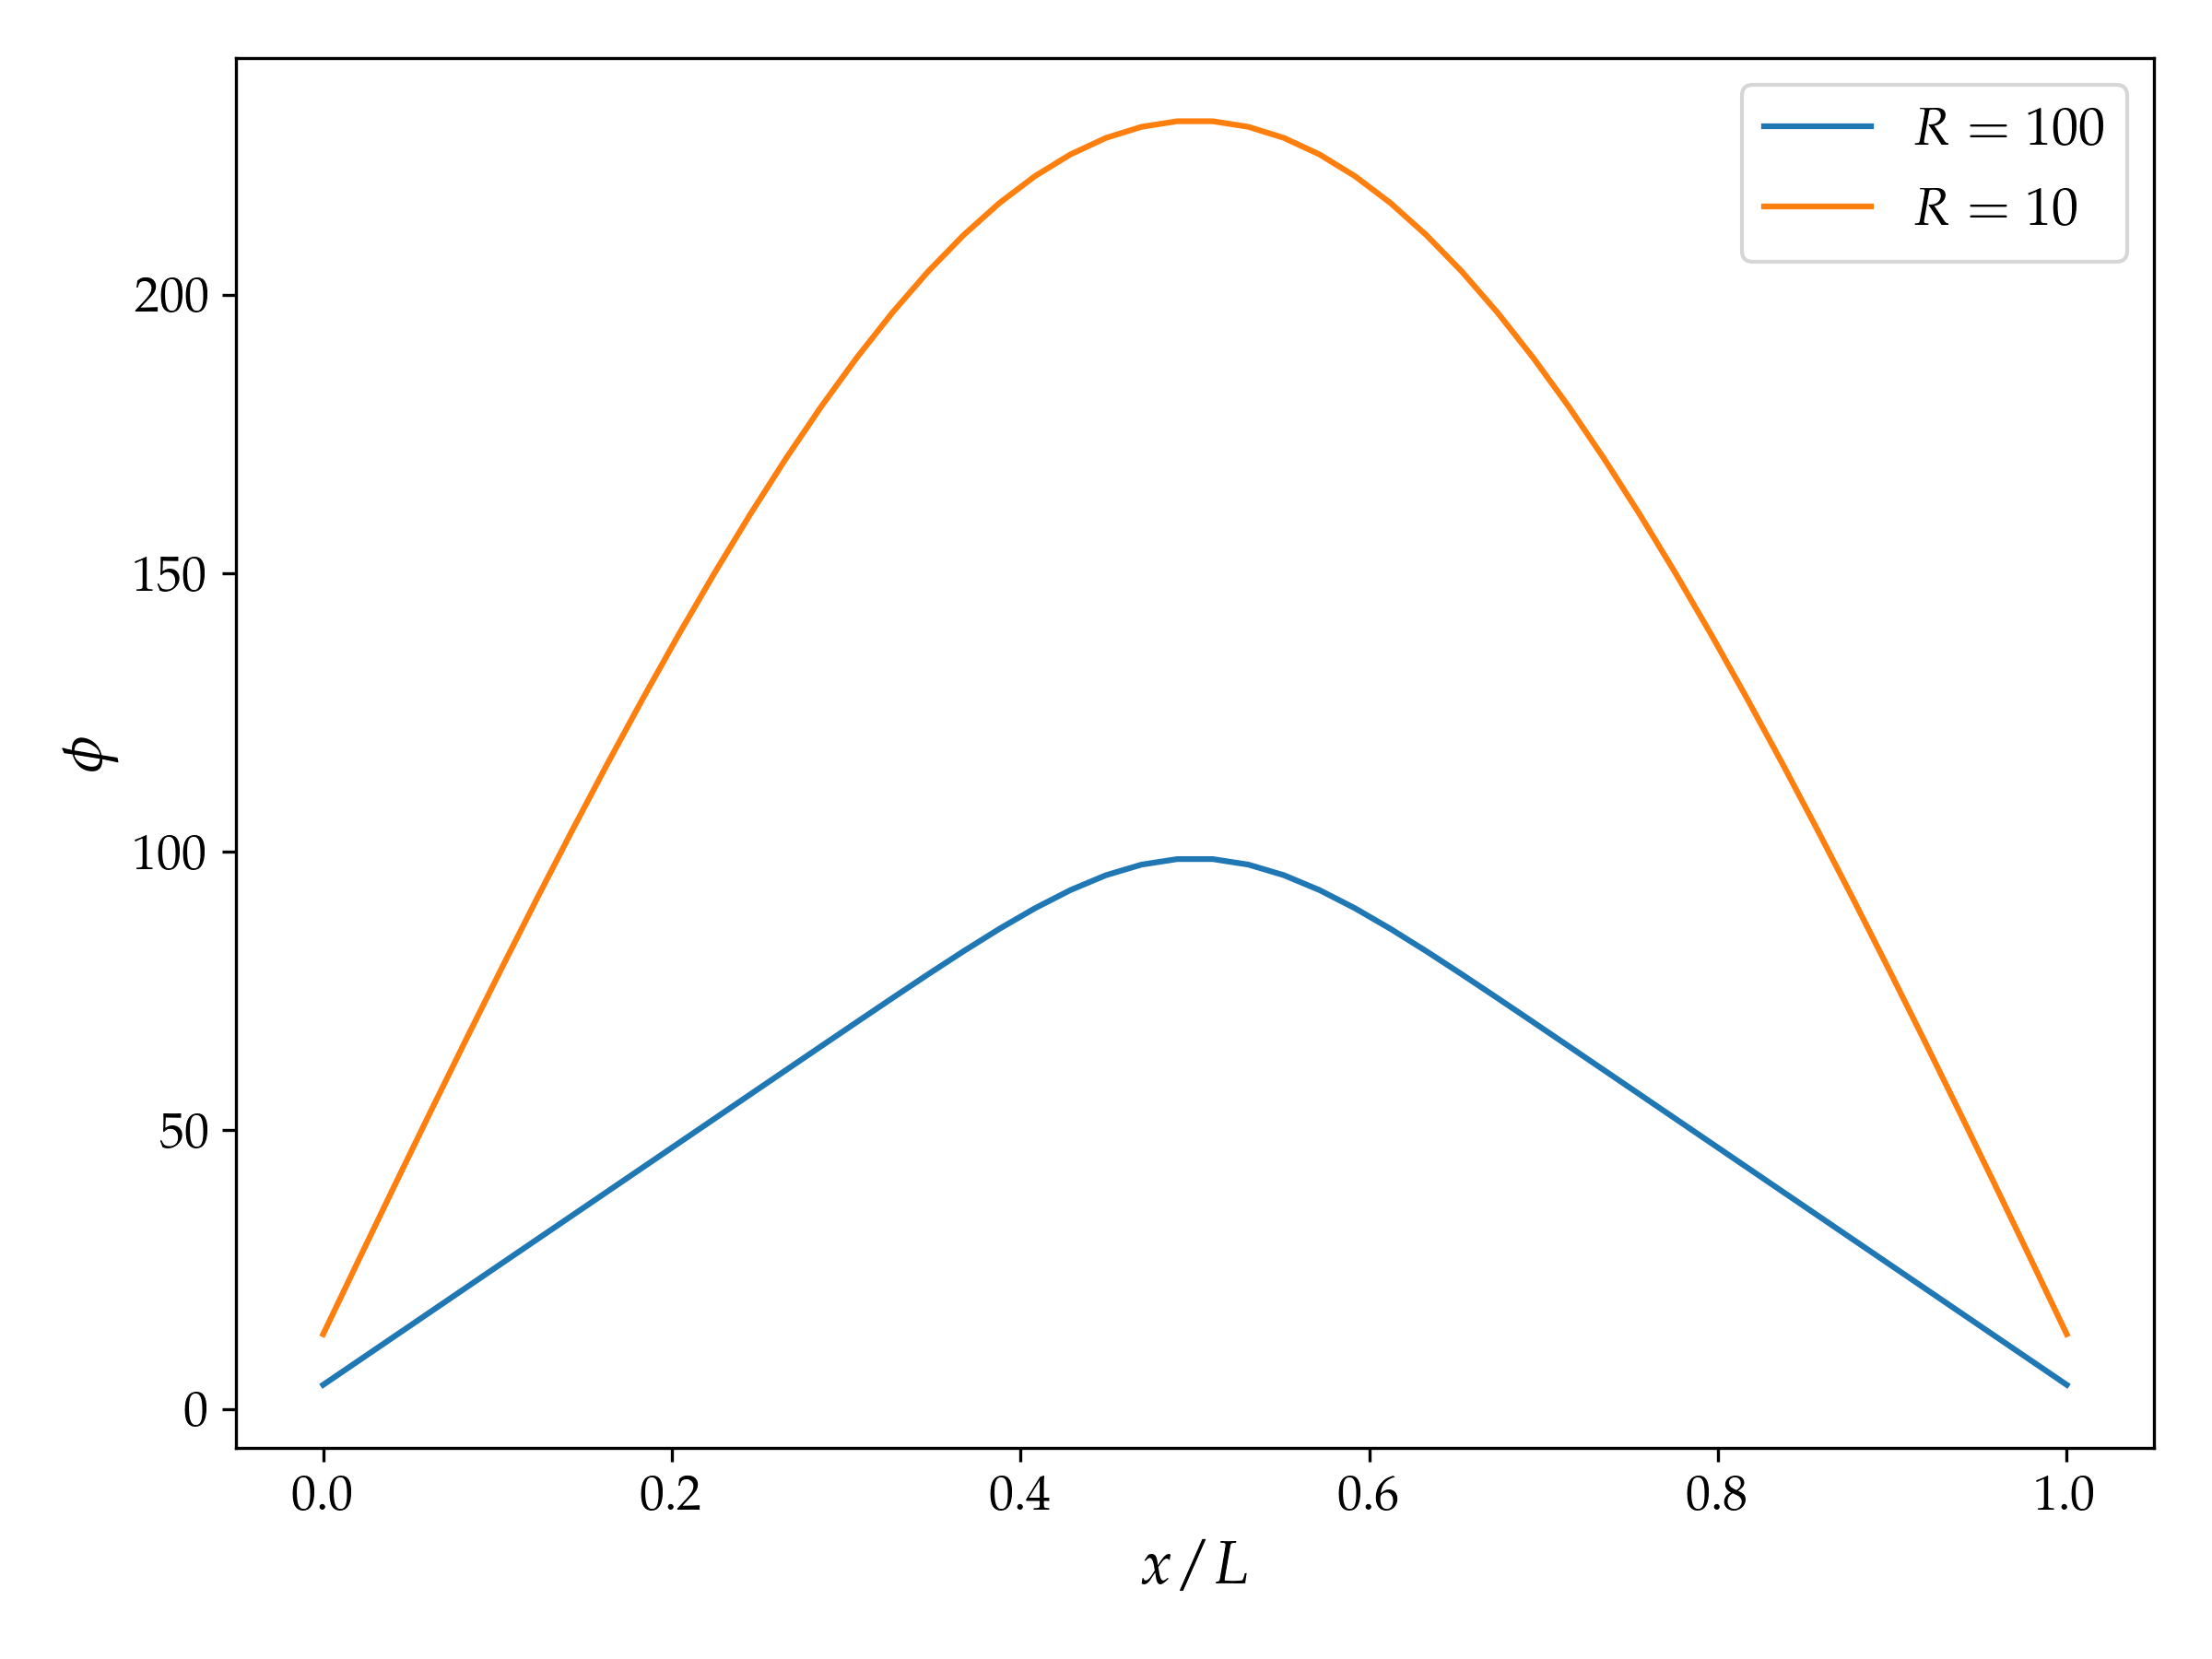
\includegraphics[width=0.7\linewidth]{images/4/poiss_sol.png}
        \captionof{figure}{Soluzione dell'equazione di Poisson $\phi$ per $R=100$ e $R=10$} 
        \label{fig: poiss_label}
    \end{center}
\end{enumerate}

\newpage


